\begin{frame}{High-performance computing --- objectives}

  \begin{itemize}
  \item Do science using the computer
    \begin{itemize}
    \item Emphasizes productivity, speed of testing new ideas, correctness
    \end{itemize}
    
  \item Science is collaborative, funding limited, software long lived
      \begin{itemize}
      \item Need readable, extensible, maintainable, portable software
      \end{itemize}
      
  \item Science is done by science students not computer scientists
      \begin{itemize}
      \item Ideally code in high-level concepts, hiding arcane computer details
      \end{itemize}

  \item Big/many calculations and/or a large user community
      \begin{itemize}
      \item Demand high-performance, efficient use of resources, robustness
      \end{itemize}
  \end{itemize}
\end{frame}

\begin{frame}{Practical high-performance computing}
  \begin{itemize}
  \item Performance is a level-1 correctness issue
  \item How to make a computer run fast?
  \item How to do this portably?
    \begin{itemize}
    \item Current machines
    \item Future machines
    \end{itemize}
  \item How to do this while maintaining productivity?
  \end{itemize}
\end{frame}

\begin{frame}{Technology trends}

  \begin{itemize}
  \item Power wall 
    \begin{itemize}
    \item Computer clock frequencies are no longer steadily increasing
    \end{itemize}

  \item Memory wall 
    \begin{itemize}
    \item Memory, communication, and disk bandwidth increasing less rapidly than compute speed
    \item New technologies (e.g., stacked memory) essential to progress
    \end{itemize}
  
  \item Parallelism is the {\bf only} path to increased performance
    \begin{itemize}
    \item Fine-grain
      \begin{itemize}
      \item instructions --- MIMD
      \item vectors --- SIMD
      \end{itemize}

    \item Medium-grain
      \begin{itemize}
      \item cores --- MIMD
      \end{itemize}

    \item Coarse-grain
      \begin{itemize}
      \item sockets, nodes --- MIMD
      \end{itemize}
    \end{itemize}

  \item Good news --- technology is delivering more fine/medium grain
    \begin{itemize}
    \item Phew!  1M-way coarse grain parallelism is too much!
    \item What to do with all those transitors?
    \end{itemize}
  \end{itemize}
\end{frame}

\begin{frame}[shrink=20]{Connecting concepts in architecture, software, and tools}

\begin{center}
\begin{tabular}{l|l|l}
{\bf Architectural}  &     {\bf Software}            &   {\bf Programming} \\
{\bf element}        &     {\bf construct}           & {\bf tool} \\ \hline
 {\it within a "core"} & & \\
 pipe-lined units    &  complex expressions, loops   & compiler, library \\
 multiple instruction& complex expresions, fat loops &           compiler \\
 simd units & loops, ops on vectors/matrices         & compiler, library \\
 & & \\
 {\it within a "node"} & & \\
 cores/thread units  &  thread/process/task          &  openmp, pthreads, tbb \\
                     &  loop nests, ops on matrices  & openmp, opencl, libraries \\
 accelerators        &   task, ops on matrices       & opencl, openacc, cuda, libs \\
 & & \\
 {\it between "nodes"} & & \\
 distributed memory & outer loops, multiple tasks, &  mpi, libraries \\ 
                    &  big matrices                & \\ \hline
\end{tabular}
\end{center}
  
\end{frame}

\begin{frame}[fragile]{Just do it!}
  \begin{itemize}
  \item Overthinking all this is counter productive
  \item Write pipelineable, vectorizable code --- more on this later
  \item Have the compiler do the work
  \end{itemize}

\begin{verbatim}

  for (int i=0; i<n; i++) {
     c[i] = a[i]*23.0 + exp(d[i]*d[i]);
  }
\end{verbatim}
\end{frame}

\begin{frame}[fragile]{Hello world vector style}
\begin{itemize}
\item Code
{\small
\begin{verbatim}
#include <iostream>

int main() {
    double a[100];
    for (int i=0; i<100; i++) a[i] = i;
    double sum = 0.0;
    for (int i=0; i<100; i++) sum += a[i];
    std::cout << sum << std::endl;
    return 0;
}
\end{verbatim}
}
\item Compilation
\begin{verbatim}
$ icpc -fast -vec_report3 sum.cc                                            
sum.cc(5): (col. 5) remark: FUSED LOOP WAS VECTORIZED.  
\end{verbatim}
\item Output ($\sum_{i=0}^{n-1} i = n(n-1)/2 = $4950)
\begin{verbatim}
$ ./a.out                                                                   
4950                        
\end{verbatim}
\end{itemize}
\end{frame}


\begin{frame}{Thinking about performance}
  \begin{itemize}
  \item What is the bottleneck
    \begin{itemize}
    \item Data motion?
    \item Instruction issue?
    \item Functional units?  
    \end{itemize}

  \item Moving data
    \begin{itemize}
    \item disk
    \item main memory
    \item some level of cache
    \item registers
    \end{itemize}
  \item Performance model
  \end{itemize}
\[
    t(n) = L + \frac{n}{B}
\]

\begin{center}
$L = $ latency, $B = $ bandwidth, $n = $ number of elements
\end{center}



\end{frame}


\begin{frame}{Hockney's $n_{1/2}$}
  \begin{itemize}
  \item How long must a loop be, or how much data must we move, in order to hit 50\% performance

\[
  \mbox{rate}(n) = \frac{n}{t(n)} = \frac{n}{L + \frac{n}{B}} = \frac{B}{\frac{B L}{n} + 1}
\]  

  \item The asymptotic rate is just

\[
   \mbox{rate}(\infty) = B
\]

  \item Hence, 

\[
   \mbox{rate}(n_{1/2}) = \frac{B}{2} \rightarrow n_{1/2} = B L
\]

  \item also

\[
   \mbox{rate}(n_{90\%}) = 0.9 B \rightarrow n_{90\%} = 9 B L
\]

  \end{itemize}
  
\end{frame}


\begin{frame}{E.g., typical message passing between processes}

    \begin{itemize}
    \item latency 5us, bandwidth 1e9 bytes/s
    \item $n_{1/2} =$ 1,000 bytes
    \item $n_{90\%}$ = 9,000 bytes
    \end{itemize}

\end{frame}

\begin{frame}{Pipelined functional units}
  \begin{itemize}
  \item Parallelism arises from overlapping stages of performing successive operations
  \item E.g., floating point a*b
    \begin{itemize}
    \item A single operation may take 3 cycles to complete (pipeline depth or latency)
    \item You can issue a new operation every cycle
    \end{itemize}
  \end{itemize}

  \begin{center}
    \begin{tabular}{ccccc}
 cycle & stage0 & stage1 & stage2 & result \\ \hline
  1    & a0*b0  &        &        & \\
  2    & a1*b1  &a0*b0   &        & \\
  3    & a2*b2  &a1*b1   & a0*b0  & \\
  4    & a3*b3  &a2*b2   & a1*b1  & a0*b0 \\
  5    & a4*b4  &a3*b3   & a2*b2  & a1*b1 \\
  \vdots    & \ldots &        &        &       \\ \hline

    \end{tabular}
  \end{center}
  
\end{frame}

\begin{frame}{Pipelined functional units}
  \begin{itemize}
  \item Serial execution 
    \begin{itemize}
    \item Wait for each result to complete
    \item The cost per operation is the pipeline depth
    \end{itemize}
  \item Pipelined execution
    \begin{itemize}
    \item $t(n) = L + n - 1 \ \ \ \mbox{(in cycles)}$
    \item $n_{1/2} = L-1$
    \item $n_{90\%} = 9*(L-1)$  \ \  9*2 = 18
    \end{itemize}
  \end{itemize}
\end{frame}

\begin{frame}[fragile]{Multiple instruction issue}
  \begin{itemize}
  \item High-end x86 can issue each cycle at least
    \begin{itemize}
    \item  One or more integer operations (e.g. inc loop counter)
    \item A test+branch operation
    \item A (simd) floating point multiply
    \item A (simd) floating point addition
    \item Two (simd) memory operations
    \end{itemize}
  \item The integer units typically have 1 cycle latency
  \item FMA --- fused multiply-add --- \verb,a*b+c-->d,
    \begin{itemize}
    \item Introduced with Haswell (\url{http://goo.gl/Bo3Rt}, \url{http://goo.gl/tePyD})
    \end{itemize}
  \item The compiler does this for you --- usually better than humans except on very tight loops.
  \end{itemize}
  
\end{frame}

\begin{frame}{SIMD (vector) operations}
  \begin{itemize}
  \item Single instruction applying operation to multiple data

\[
  \begin{pmatrix}a_0\\a_1\\a_2\\a_3\end{pmatrix}
  *
  \begin{pmatrix}b_0\\b_1\\b_2\\b_3\end{pmatrix}
  \rightarrow 
  \begin{pmatrix}a_0 * b_0\\a_1*b_1\\a_2*b_2\\a_3*b_3\end{pmatrix}
\]

  \item Older x86 --- SSE --- 2 doubles (128 bit)
  \item Newest x86 --- AVX(2) --- 4 doubles (256 bit), predicates, special functions, gather, scatter
  \item MIC x86 --- LRBNI --- 8 doubles (512bit), predicates, special functions, gather, scatter
  \item Zillions of different operations (\url{http://goo.gl/D0d7t})
  \\
  \item Operations are pipelined 

  \item $n_{90\%} = 9*W*(L-1) =$108 with $W$=4 (width) and $L=$4 (latency)

  \end{itemize}
  
\end{frame}

\begin{frame}{Serial scalar v.s. pipelined SIMD performance}

  \begin{itemize}
  \item Serial scalar computation produces 1 result every $L$ cycles
  \item Pipelined SIMD produces $W$ results every cycle
  \item Pipelined is $W L$ times faster which is 16 with $W=L=$4
  \item Allowing for 2 operations per cycle (*,+) this becomes $32$
  \item I.e., worst case serial, non-vector code can be 32x slower!!!!
  \\  
  
  \item Whenever some twit talks about GPGPUs being 100+ times faster
    than a CPU ask about how well vectorized (and threaded) the CPU
    code was.

  \end{itemize}

\end{frame}

\begin{frame}[fragile]{Example performance --- DAXPY}

  \begin{itemize}
  \item Measure cycles/iteration of this loop as a function of $n$

\begin{verbatim}

  for (int i=0; i<n; i++) {
      y[i] = a*x[i] + y[i];
  }

or from VML

  cblas_daxpy (n, a, x, 1, y, 1);

\end{verbatim}

  \item What are you expecting to see?
  \end{itemize}
  
\end{frame}

\begin{frame}{Example performance --- DAXPY}

  \begin{figure}
      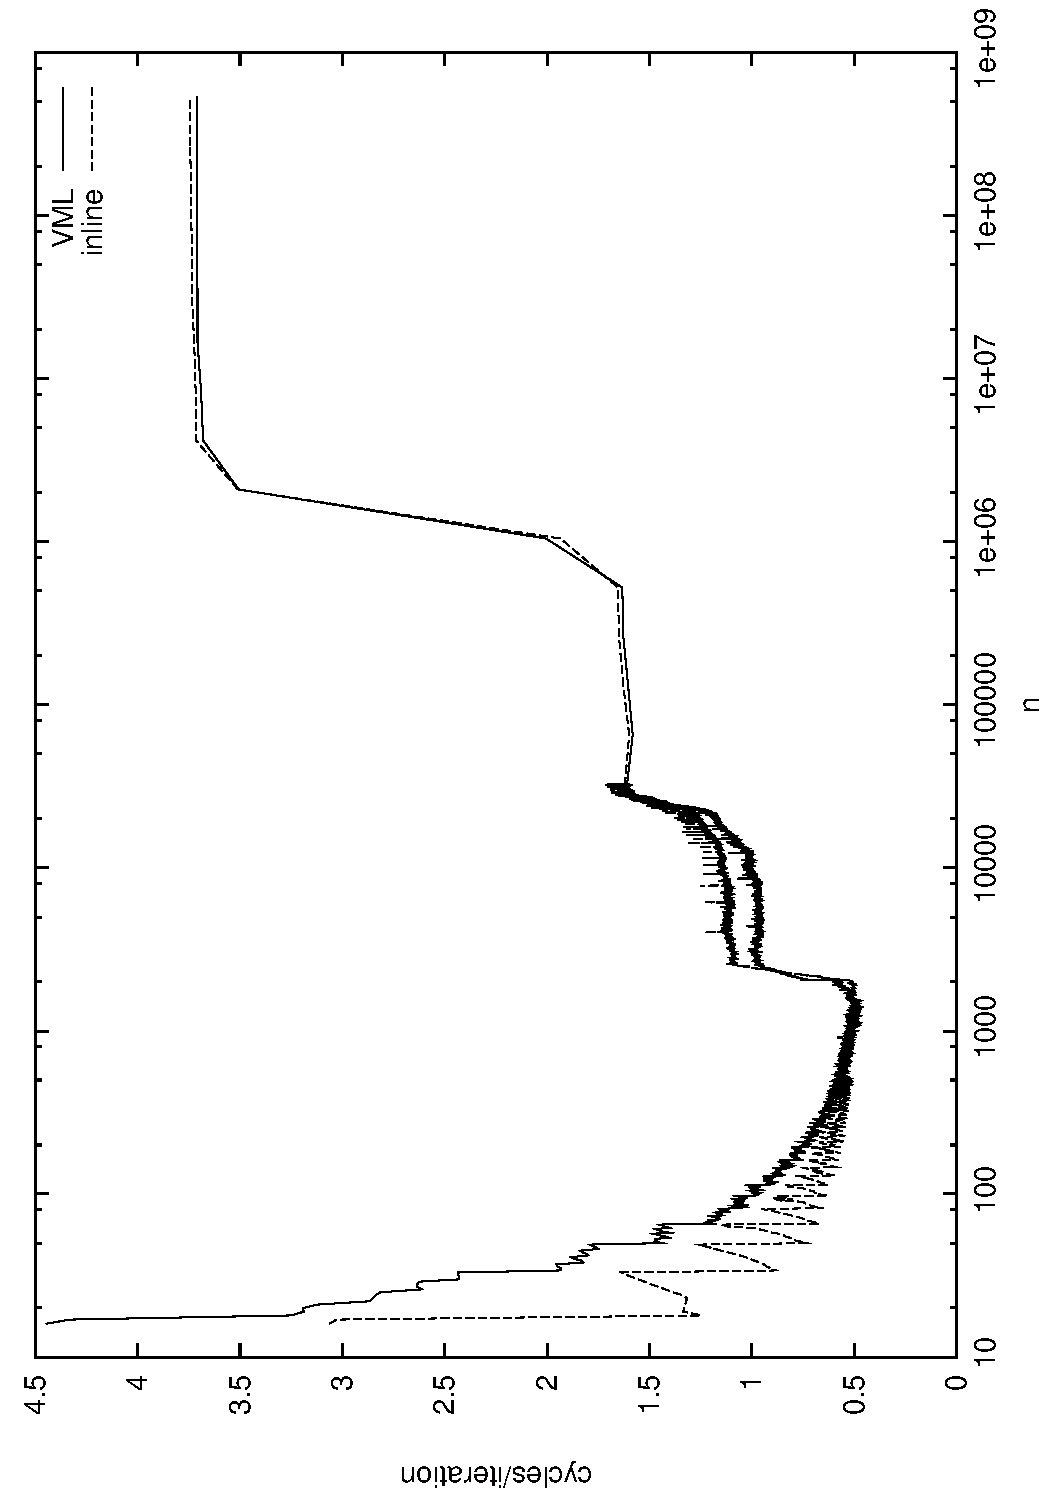
\includegraphics[width=0.65\linewidth,angle=270]{img/daxpy.pdf}
  \end{figure}

\end{frame}

\begin{frame}[fragile]{DAXPY performance analysis}
  \begin{itemize}
  \item Each element needs 2 loads, *, +, store (unrolling offsets increment+branch)
  \item Can only do 2 memory operations per cycle \ldots need 2 cycles
  \item AVX SIMD is 4 wide
  \item Hence, 4 iterations per 2 cycles = 0.5 cycles/iter at best
  \item L1 = 32KB (4096 dbl), 48 bytes/cycle \\
  (capable of 64 bytes/cycle?)
  \item L2 = 256KB (32768 dbl), ~21 bytes/cycle
  \item L3 = 8MB (1M dbl), ~14.8 bytes/cycle
  \item main memory, ~6.4 bytes/cycle
  \end{itemize}
  
\end{frame}

\begin{frame}[fragile]{DAXPY performance analysis}
  \begin{itemize}
  \item Lesson --- cache fast, memory slow (latency even more so)
  \\
  \ 
  \item Assignment --- predict then measure performance of
\begin{verbatim}
  for (int i=0; i<n; i+=4) {
     y[i] = a*x[i] + y[i];
}
\end{verbatim}
  (remember to account for reduced number of elements in perf. anal.)
  \item Assignment --- what if stride is 4096 instead of 4?
  \end{itemize}
  
\end{frame}

\begin{frame}{Read the documentation --- really!}

  \begin{itemize}
  \item The tools do a {\bf lot} more than most people realize.
  \item Will introduce lots of valuable concepts and techniques.
  \item Read the release notes with every new version.
  \item Intel developer zone
{\tiny
        \url{http://software.intel.com/}
}
  \item Intel compilers {\tiny
        \url{http://software.intel.com/en-us/intel-compilers}
}
  \item Intel composer software suite
{\tiny
        \url{http://software.intel.com/en-us/articles/intel-c-composer-xe-2011-documentation}
}
  \item Intel C++ compiler
{\tiny
        \url{http://software.intel.com/sites/products/documentation/doclib/stdxe/2013/composerxe/compiler/cpp-lin/index.htm}
}
  \item Getting started with auto-vectorization
{\tiny
        \url{http://software.intel.com/sites/products/documentation/doclib/stdxe/2013/composerxe/tutorials/lin/cmp_vec_c/index.htm}
}
  \end{itemize}

\end{frame}

\begin{frame}{More Intel links}

  \begin{itemize}
  \item Go parallel portal \url{http://go-parallel.com/}
  \item Learning lab \url{http://software.intel.com/en-us/intel-learning-lab/}
  \item Vectorization \url{http://software.intel.com/en-us/intel-vectorization-tools/}
  \item Evaulation guide portale \url{http://software.intel.com/en-us/evaluation-guides/}
  \item Parallel magazine \url{http://software.intel.com/en-us/intel-parallel-universe-magazine/}
  \item OpenCL \url{http://software.intel.com/en-us/vcsource/tools/opencl-sdk}
\item MxM using MKL \url{http://software.intel.com/sites/products/documentation/doclib/mkl_sa/11/tutorials/mkl_mmx_c/tutorial_mkl_mmx_c.pdf}

  \end{itemize}
    
\end{frame}


\begin{frame}[fragile]{Non-vectorizable loops}
  \begin{itemize}
\item Dependencies between iterations
\begin{verbatim}
  for (int=1; i<n; i++) a[i-1] = 3*a[i];
\end{verbatim}
\item Dependencies through memory
\begin{verbatim}
  void f(int n double *a, double* b) {
    for (int=0; i<n; i++) a[i] = b[i];
  }
\end{verbatim}
\item Dependencies through iteration index or count
\begin{verbatim}
  for (int i=0; i<n; i++) {if (a[i] > 1) n++;}
  for (int i=0; i<n; i++) {if (a[i] > 1) i++;}
\end{verbatim}
\item Calls to non-inline functions (math library exceptions)
\item If-tests that don't resolve to vector merge  
  \end{itemize}
\end{frame}

\begin{frame}[fragile]{Passing your knowledge to the compiler}
  \begin{itemize}
  \item \verb+#pragma ivdep+ --- ignore vector dependencies
  \item \verb+restrict+
  \item \verb+-fargument-noalias+ ---  function arguments cannot alias each other, but they can alias global storage
  \item \verb+-fargument-noalias-global+ ---  function arguments cannot alias each other or global storage
  \item \verb+#pragma loop count (n)+ --- advises the compiler of the typical trip count of the loop.
  \item \verb+#pragma vector always+ --- always vectorize if safe regardless of if performance improvement expected
  \item \verb+#pragma vector align+ --- asserts that data within the following loop is aligned (to a 16 byte boundary, for SSE instruction sets)
  \item \verb+#pragma novector+ --- asks the compiler not to vectorize a particular loop.
  \end{itemize}
\end{frame}

\begin{frame}[fragile]{Passing your knowledge to the compiler}
  \begin{itemize}
  \item \verb+#pragma vector nontemporal+ --- gives a hint to the compiler that data will not be reused, and therefore to use streaming stores that bypass cache.
  \item \verb+#pragma simd+ --- Lots of options. Forces vectorization even if it is unsafe.
  \item \verb+__attribute__((vector))+ and \verb+__declspec(vector)+ --- Vectorization of functions when definition is not available for inlining.
  \end{itemize}
\end{frame}

\begin{frame}{Monte Carlo Example}

  \begin{itemize}
  \item Metropolis Monte Carlo
    \begin{itemize}
    \item General and powerful algorithm for multi-dimensional integration
    \item Abuse it to create a simple test code that reflects real applications
    \end{itemize}

  \item Compute average value of $x$ sampled from the normalized probably distribution function $e^{-x}$, i.e., 

\[
    \langle x \rangle = \frac{\int_0^{\infty} x e^{-x} dx}{\int_0^{\infty} e^{-x} dx} = 1
\]


  \end{itemize}
\end{frame}

\begin{frame}[fragile]{Monte Carlo Example - II}

  \begin{itemize}
  \item Starting from uniform random numbers in $[0,1)$ use Metropolis
    algorithm to sample from $e^{-x}$
  \item Approxmate infinity as 23 ($exp(-23) =$1e-10)
  \item Algorithm
\begin{verbatim}
   x = 23.0*rand() // initialize
   while (1) {
      xnew = 32.0*rand();
      if (exp(-xnew) > exp(-x)*rand()) x = xnew;
   }
\end{verbatim}
  \item Asymptotically, $x$ is sampled from $exp(-x)$ (with some correlation between successive values)
  \end{itemize}

\end{frame}

\begin{frame}[fragile]{Monte Carlo Example - II}
  \begin{itemize}
  \item Intel(R) Xeon(R) CPU E5-2687W
    \begin{itemize}
    \item \verb+mc0+ --- 71.2 cycles/point
    \item \verb+mc1+ --- 71.8
    \item \verb+mc2+ --- 76.2
    \item \verb+mc3+ --- 54.3
    \item \verb+mc4+ --- 18.0
    \item \verb+mc5+ --- 14.8
    \end{itemize}
  \item Intel(R) Xeon(R) CPU E5645 (Hokiespeed)
  \end{itemize}
\end{frame}

\begin{frame}{Variational Monte-Carlo Example}

  \begin{itemize}
  \item Uses Metropolis algorithm to sample points distributed according to $\psi^2$ for the helium atom and the Hylleraas wave function 
\[
\psi(r_1, r_2, r_{12}) = (1 + \tfrac{1}{2} r_{12}) e^{-2 (r_1 + r_2)}
\]
  \item Variational since $\langle E_L \rangle >= E_0$ where $E_L = (\hat{H} \psi)/\psi$
  \item Computes $\langle r_1 \rangle$, $\langle r_2 \rangle$, $\langle r_{12} \rangle$
  \end{itemize}
  
\end{frame}
 
\begin{frame}{Assignments for vector programming}

  \begin{enumerate}
  \item Read (at least skim) all the compiler reference manual \\
  Pay special attention to the autovectorization section
  \item Work through the autovectorization getting started
  \item Examine the model matrix multiplication code
  \item Understand each of the Monte Carlo code versions and reproduce performance
  \item Tune a kernel relevant to you (modify bench.cc to measure performance)
  \end{enumerate}
  
\end{frame}


\begin{frame}{Shared-memory programming beyond data-parallel OpenMP}

  \begin{itemize} 

  \item OpenMP \\
{\tiny \url{https://computing.llnl.gov/tutorials/openMP/}} \\

{\tiny \url{https://iwomp.zih.tu-dresden.de/downloads/omp30-tasks.pdf}}\\

{\tiny \url{http://www.cs.utah.edu/~mhall/cs4961f11/}}\\

{\tiny \url{http://www.cs.utah.edu/~mhall/cs4961f11/CS4961-L9.pdf}}\\

\item Pthreads\\

{\tiny \url{https://computing.llnl.gov/tutorials/pthreads/ }}\\

{\tiny \url{http://www.yolinux.com/TUTORIALS/LinuxTutorialPosixThreads.html}}\\

{\tiny \url{http://cs.gmu.edu/~white/CS571/pthreadTutorial.pdf}}\\

\item TBB \\

{\tiny \url{http://www.inf.ed.ac.uk/teaching/courses/ppls/TBBtutorial.pdf}}\\

{\tiny \url{http://stackoverflow.com/questions/13446434/tbb-beginner-tutorial}}\\

{\tiny \url{http://software.intel.com/sites/products/documentation/doclib/tbb\_sa/help/index.htm\#reference/reference.htm}}

\end{itemize}
  
\end{frame}

\begin{frame}{Spinlocks v.s. mutexes}

  \begin{itemize}
  \item Spinlocks
    \begin{itemize}
    \item Fastest with low contention and no false sharing
    \item Low resource use (minimally one cache line)
    \item Potentially very slow under contention, in virtual machines, oversubscribed
    \item Spinning threads can saturate memory and slow everything
    \end{itemize}
  \item Mutexes
    \begin{itemize}
    \item Thread scheduler blocks waiting threads
    \item Usually slower than spinlocks in low contention 
    \item Scale well under contention, in virtual machines, oversubscription
    \end{itemize}
  \item Recommendations
    \begin{itemize}
    \item Use trusted implementation of higher-level concept\\
          (e.g., thread-safe containers)
    \item Think tasks, not threads
    \item Avoid heavily contested critical sections
    \item Use mutexes; try spinlocks if performance is poor
    \end{itemize}
\end{itemize}
\end{frame}

\begin{frame}[fragile]{Critical section issues}
  \begin{itemize}
  \item Fairness --- not guaranteed but often assumed
  \item Correctly updating shared data structures is not easy
    \begin{itemize}
    \item \verb+volatile+ --- does not solve the underlying problem but is useful to get the compiler to help \\
{\tiny \url{http://www.hpl.hp.com/personal/Hans_Boehm/c++mm/faq.html}}\\
{\tiny \url{http://software.intel.com/en-us/blogs/2007/11/30/volatile-almost-useless-for-multi-threaded-programming}}\\
{\tiny \url{http://www.drdobbs.com/cpp/volatile-the-multithreaded-programmers-b/184403766}}
    \item Need memory fences and compile/run time barriers to instruction migration
    \item Pthread routines provide these --- home grown assembly probably does not
    \item STL structures cannot be made volatile --- but may not need to be
    \end{itemize}
  \end{itemize}
\end{frame}


\begin{frame}{Other options}
  \begin{itemize}
  \item Condition variables
  \item Fair, scalable synchronization\\
\url{http://dl.acm.org/citation.cfm?id=103729}
  \item Again, think tasks not threads
  \end{itemize}
\end{frame}

\begin{frame}{Intel Thread Building Blocks}


  
\end{frame}
 
